%!TEX root = ../thesis.tex
\subsection{Automatic Generation Pipeline}
\label{mixt_pipeline}

To generate mixed media tutorials, tools can either help authors create new tutorials (e.g., \cite{Grabler:2009jj}), or they can reformat existing video tutorials into step-by-step videos (e.g., \cite{Pongnumkul:2011ju}). Our system adopts the former approach and extends Grabler \ea's system for generating static tutorials from demonstration to include videos \cite{Grabler:2009jj}. Producing mixed media tutorials requires three steps (Figure~\ref{fig:mixt_pipeline}). First, MixT captures an application command log, screencast video and an input device event log and synchronizes them. Second, MixT generates appropriate media files and descriptions: it transforms the log into text instructions, segments the video into steps, and identifies active UI regions, which inform the different video playback modes. Finally, MixT composes the text, images, and video into one document and adds mouse interactions as visualizations on top of the videos. For each step in the tutorial, MixT produces the three video formats and one representative step image.

\begin{figure*}[t]
  \centering
  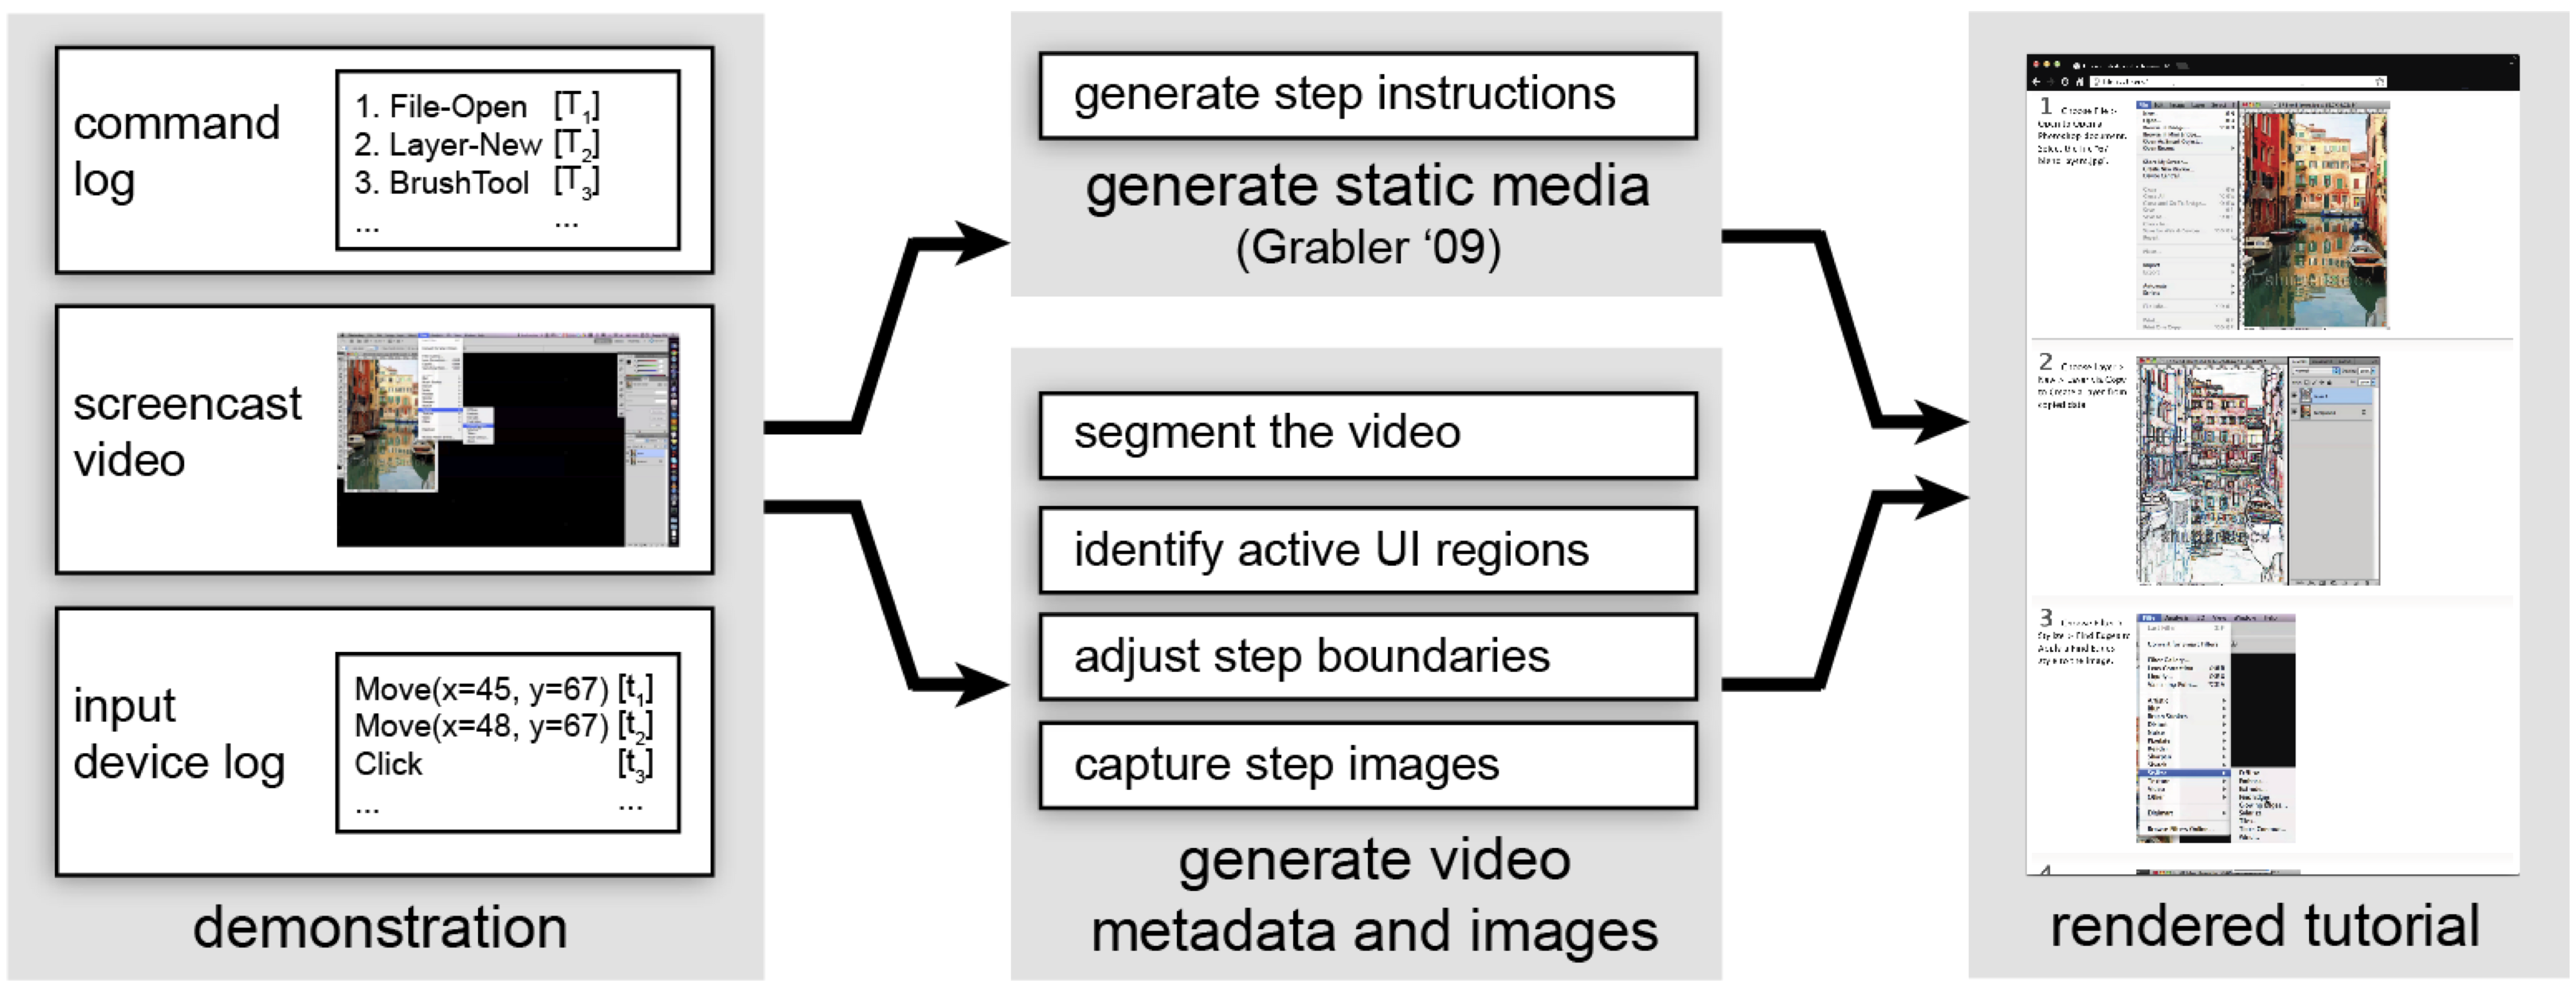
\includegraphics[width=\textwidth]{\mixt/fig/mixt_pipeline/mixt_pipeline}
  \caption{MixT generates tutorials from video and log files.}
  \label{fig:mixt_pipeline}
\end{figure*}

\subsubsection{Recording the Demonstration}
MixT records three different time-synchronized data streams during a demonstration: a history of executed application commands; a trace of mouse events; and screencapture video of the entire application interface. To capture application commands, such as opening a file, selecting a region, or hiding a layer, we use Tutorial Builder\footnote{http://labs.adobe.com/technologies/tutorialbuilder/}, a freely available Photoshop plug-in that records commands and transforms them into text instructions through text templates. To synchronize Tutorial Builder output with the screencast video and mouse streams, we timestamp the command log during the user demonstration. We obtain mouse event traces on Apple’s OS X operating system through the Event Taps\footnote{http://developer.apple.com/library/mac/\#documentation/Carbon/\newline
Reference/QuartzEventServicesRef/Reference/reference.html} API, which observes system-wide input events. We record full-screen video with the commercial Camtasia application\footnote{http://www.techsmith.com/camtasia.html}.

\subsubsection{Generating Video Metadata and Step Images}
After acquiring the time-synchronized data, there are three technical challenges:

1) Segmenting the video into steps: MixT segments the screencapture video into individual steps based on the timestamps for individual commands in the command log. We map each command Cmdi with timestamp Ti to a video segment that starts at Ti and ends at Ti+1.

2) Identifying active UI regions for zooming and cropping: MixT uses zooming and cropped side-by-side views to preserve legibility for videos at small video frame sizes. To create these specialized views, MixT needs metadata describing the relevant pixel coordinates for each step. Each command in the command log contains information about the logical UI regions that are involved (e.g., the toolbar, a dialog box, or the canvas). However, many commands can be invoked in multiple ways. For example, the New-Layer command can be accessed through the application menu, or an icon on the Layer Palette. Therefore, MixT must find and select the correct UI regions from a set of candidates. MixT first uses pixel-based template matching \cite{Pongnumkul:2011ju} to locate these areas on the screen. MixT then identifies the active UI region by inspecting the mouse event log to see which candidate region received a mouse click at the recorded timestamp Ti of Cmdi. If there are no mouse clicks detected (e.g., a command invoked via keyboard shortcut), MixT treats the entire frame as the active UI region to ensure the application response is visible in the video.

3) Adjusting segmentation boundaries: While segmenting the video based on the command log timestamps produces a reasonable rough alignment between steps and video segments, there are some cases where a command is recorded after important UI events have taken place. One typical case is menu navigation. For example, to use the Replace Color operation, the user moves from the Image menu through the Adjustment sub menu to the Replace Color option. The entire traversal sequence is relevant information as it explains how to reach the menu item. However, the command log only records Replace Color when the operation is invoked, which means that a video segment generated based solely on command timestamps would not include the menu traversal.

MixT adjusts step boundaries by leveraging template matching and the mouse event log. To compute the start time of the tutorial step for Cmdi, our algorithm starts at the command timestamp Ti, looks backward for all mouse clicks that occur within any visible candidate UI region for the command (e.g., menus, panels, toolbar) between Ti and the recorded Ti-1 of the previous command, and sets the adjusted start time of the step Ti’ to the time of the earliest mouse click. Adjusting step boundaries in this manner ensures that the step video clip shows all the relevant actions associated with the command.

4) Capturing screenshots and after images: Finally, in order to generate a representative static image for each step, MixT selects the most informative frame of UI interaction from the video. For example, if the step changes the layer blend mode, we show an image of the expanded blend mode menu where the appropriate option is highlighted. If the command involves a dialog box, we show the final frame when the dialog is visible. To do so, MixT selects the last frame that includes any candidate UI region within the duration of the step [Ti’, Ti+1’] and crops the frame to the UI region to produce the representative static image. Furthermore, MixT also captures the state of the canvas from the last frame of the step as an “after” image that helps viewers understand how the canvas was affected.

The MixT video analysis is implemented in MATLAB. In our dataset of nine test tutorials (see Table 2), the average duration of a step video is 12.4 seconds – our analysis takes an average of 6.3 seconds to process each step.

\subsubsection{Composing the Mixed Tutorial}
The step-by-step mixed-media tutorial with text instructions, structured screencast video, and step images is composed and presented in a web interface. The MixT tutorial viewer is implemented with standard Web technologies (HTML5, CSS3, and JavaScript) so it can be easily deployed online. In particular, all video compositing and matting is done in real-time using HTML5 video. Just-in-time compositing enables users to change viewing options on the fly without pre-rendering multiple video presentations. For example, during the video playback users can choose to show the enhanced mouse movement inside its frame for additional detail of a brush stroke, or disable the effect and focus on the incremental change on a canvas in real-time.
